\chapter{Iterazione 0}
\section{Introduzione e panoramica del sistema}
Il sistema che verrà implementato in questo progetto di studio si occuperà della gestione di un centro di immersioni, noto anche come \emph{diving center} o \emph{dive center}. Un centro di immersione è una struttura che fornisce supporto, attrezzatura e corsi per la pratica delle attività subacque. Un centro di immersione fornisce principalmente tre tipi di servizi:
\begin{itemize}
    \item Immersioni guidate.
    \item Noleggio attrezzatura.
    \item Scuola di immersione.
\end{itemize}
Per immersione guidata si intende un'immersione effettuata in gruppo o singolarmente insieme a guide subacquee addestrate, esperte e a conoscenza dei punti di immersione più importanti ed interessanti. Questa soluzione è ottimale quando ci si vuole immergere in luoghi non conosciuti o in parchi marini protetti per cui è necessaria un'autorizzazione e una guida. Inoltre il centro diving offre i servizi di accompagnamento e assistenza, di trasposto con imbarcazioni o gommoni, che permettono l'entrata e l'uscita dall'acqua con praticità e comfort.
\\
Il focus del nostro progetto sarà la gestione e l'organizzazione efficiente delle immersioni guidate e la gestione del noleggio attrezzatura, non verrà incluso l'insegnamento della pratica subacquea.
\\
Un centro di immersione ha una disponibilità limitata di barche e guide per cui ha la possibilità di effettuare un numero limitato di escursioni durante una giornata. Il sistema che verrà sviluppato si occuperà di organizzare al meglio l'allocazione delle risorse disponibili affinchè un numero maggiore di persone possa parteciparvi. Spesso le persone che vogliono partecipare a questo tipo di escursioni si trovano in gruppo, per cui è necessario ottimizzare l'allocazione delle risorse disponibili, che in questo caso costituiscono i posti disponibili in barca, con il vincolo di mantenere intatti i gruppi.
\\
Il sistema implementato rappresenterà un centro di immersione: si occuperà della gestione delle risorse (barche, escursioni, attrezzatura disponibile) e della gestione delle prenotazioni delle escursioni da parte degli utenti.
\section{Requisiti funzionali e analisi dei casi d'uso}

In questa sezione verranno introdotti i requisiti funzionali del sistema attraverso l'utilizzo dei casi d'uso.
\\Lo schema UML dei casi d'uso viene riportato in Figura~\ref{fig:casiduso}.

\begin{figure}[!ht]
    \centering
    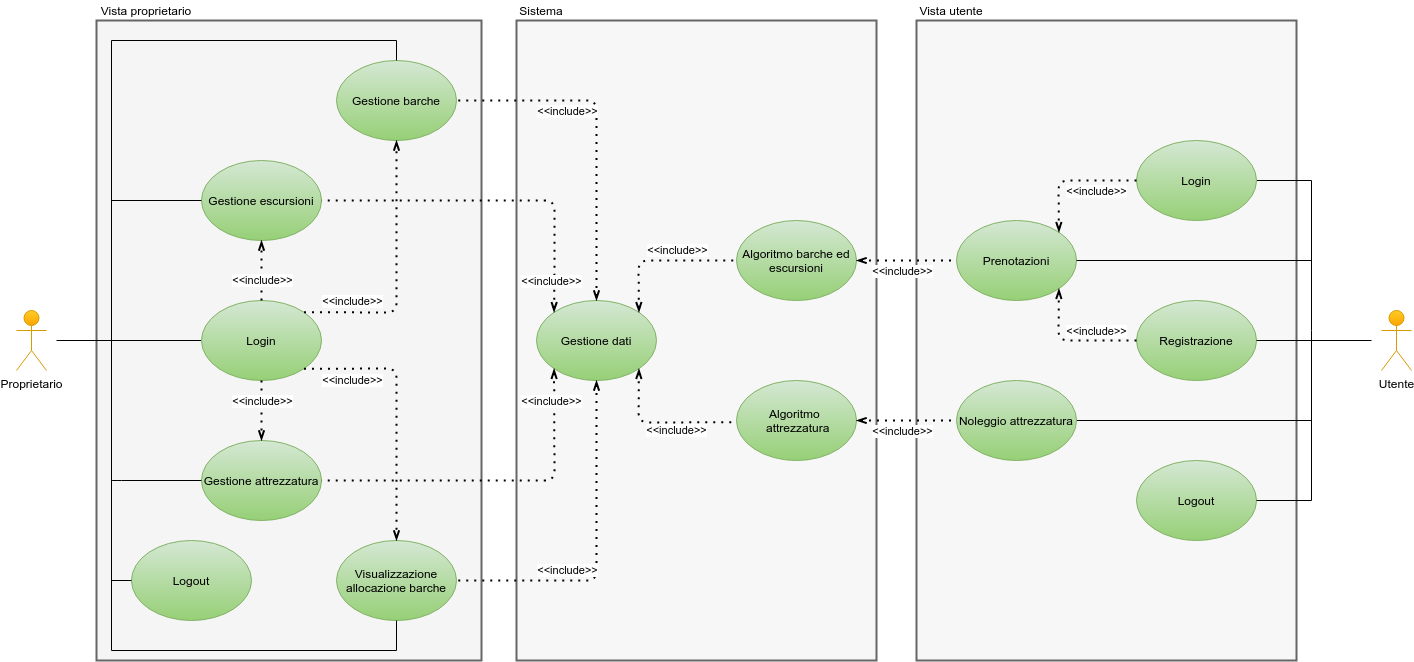
\includegraphics[width=\textwidth]{UMLcasiduso_v5.png}
    \caption{Diagramma UML dei casi d'uso}\label{fig:casiduso}
\end{figure}

\section{Requisiti non funzionali}
Il progetto verrà sviluppato tenendo in considerazione anche alcuni requisiti non funzionali, quali la manutenibilità, l'efficienza e l'usabilità.
Il requisito di manutenibilità verrà rispettato mediante l'implementazione di tutte le risorse persistenti ovvero barche, orari e date escursioni, attrezzatura. In questo modo anche se dovessero cambiare nel futuro alcune condizioni sarà facile per il proprietario rifletterle all'interno del software.
Il requisito dell'efficienza è l'obiettivo del progetto, ovvero l'allocazione ottimale delle risorse disponibili, i posti presenti nelle barche.
L'usabilità è garantita dalla decisione di sviluppare il programma attraverso un applicazione Android, di facile utilizzo sia per gli utenti che per il proprietario. In base alla topologia (Figura~\ref{fig:topologia}) è possibile notare che il database verrà ospitato da un hosting online e quindi sarà sempre possibile, mediante cellulare, accedere a tutte le funzionalità dell'applicazione.

\newpage

\section{Topologia del sistema}
La topologia  del sistema mostrata in Figura~\ref{fig:topologia} evidenzia come sia gli utenti che il proprietario accedono alla piattaforma tramite app Android.
\\Questa mette a disposizione un set di API REST con cui è possibile accedere alle funzionalità dell'applicazione che salverà i dati su un database online.

\begin{figure}[hb]
    \centering
    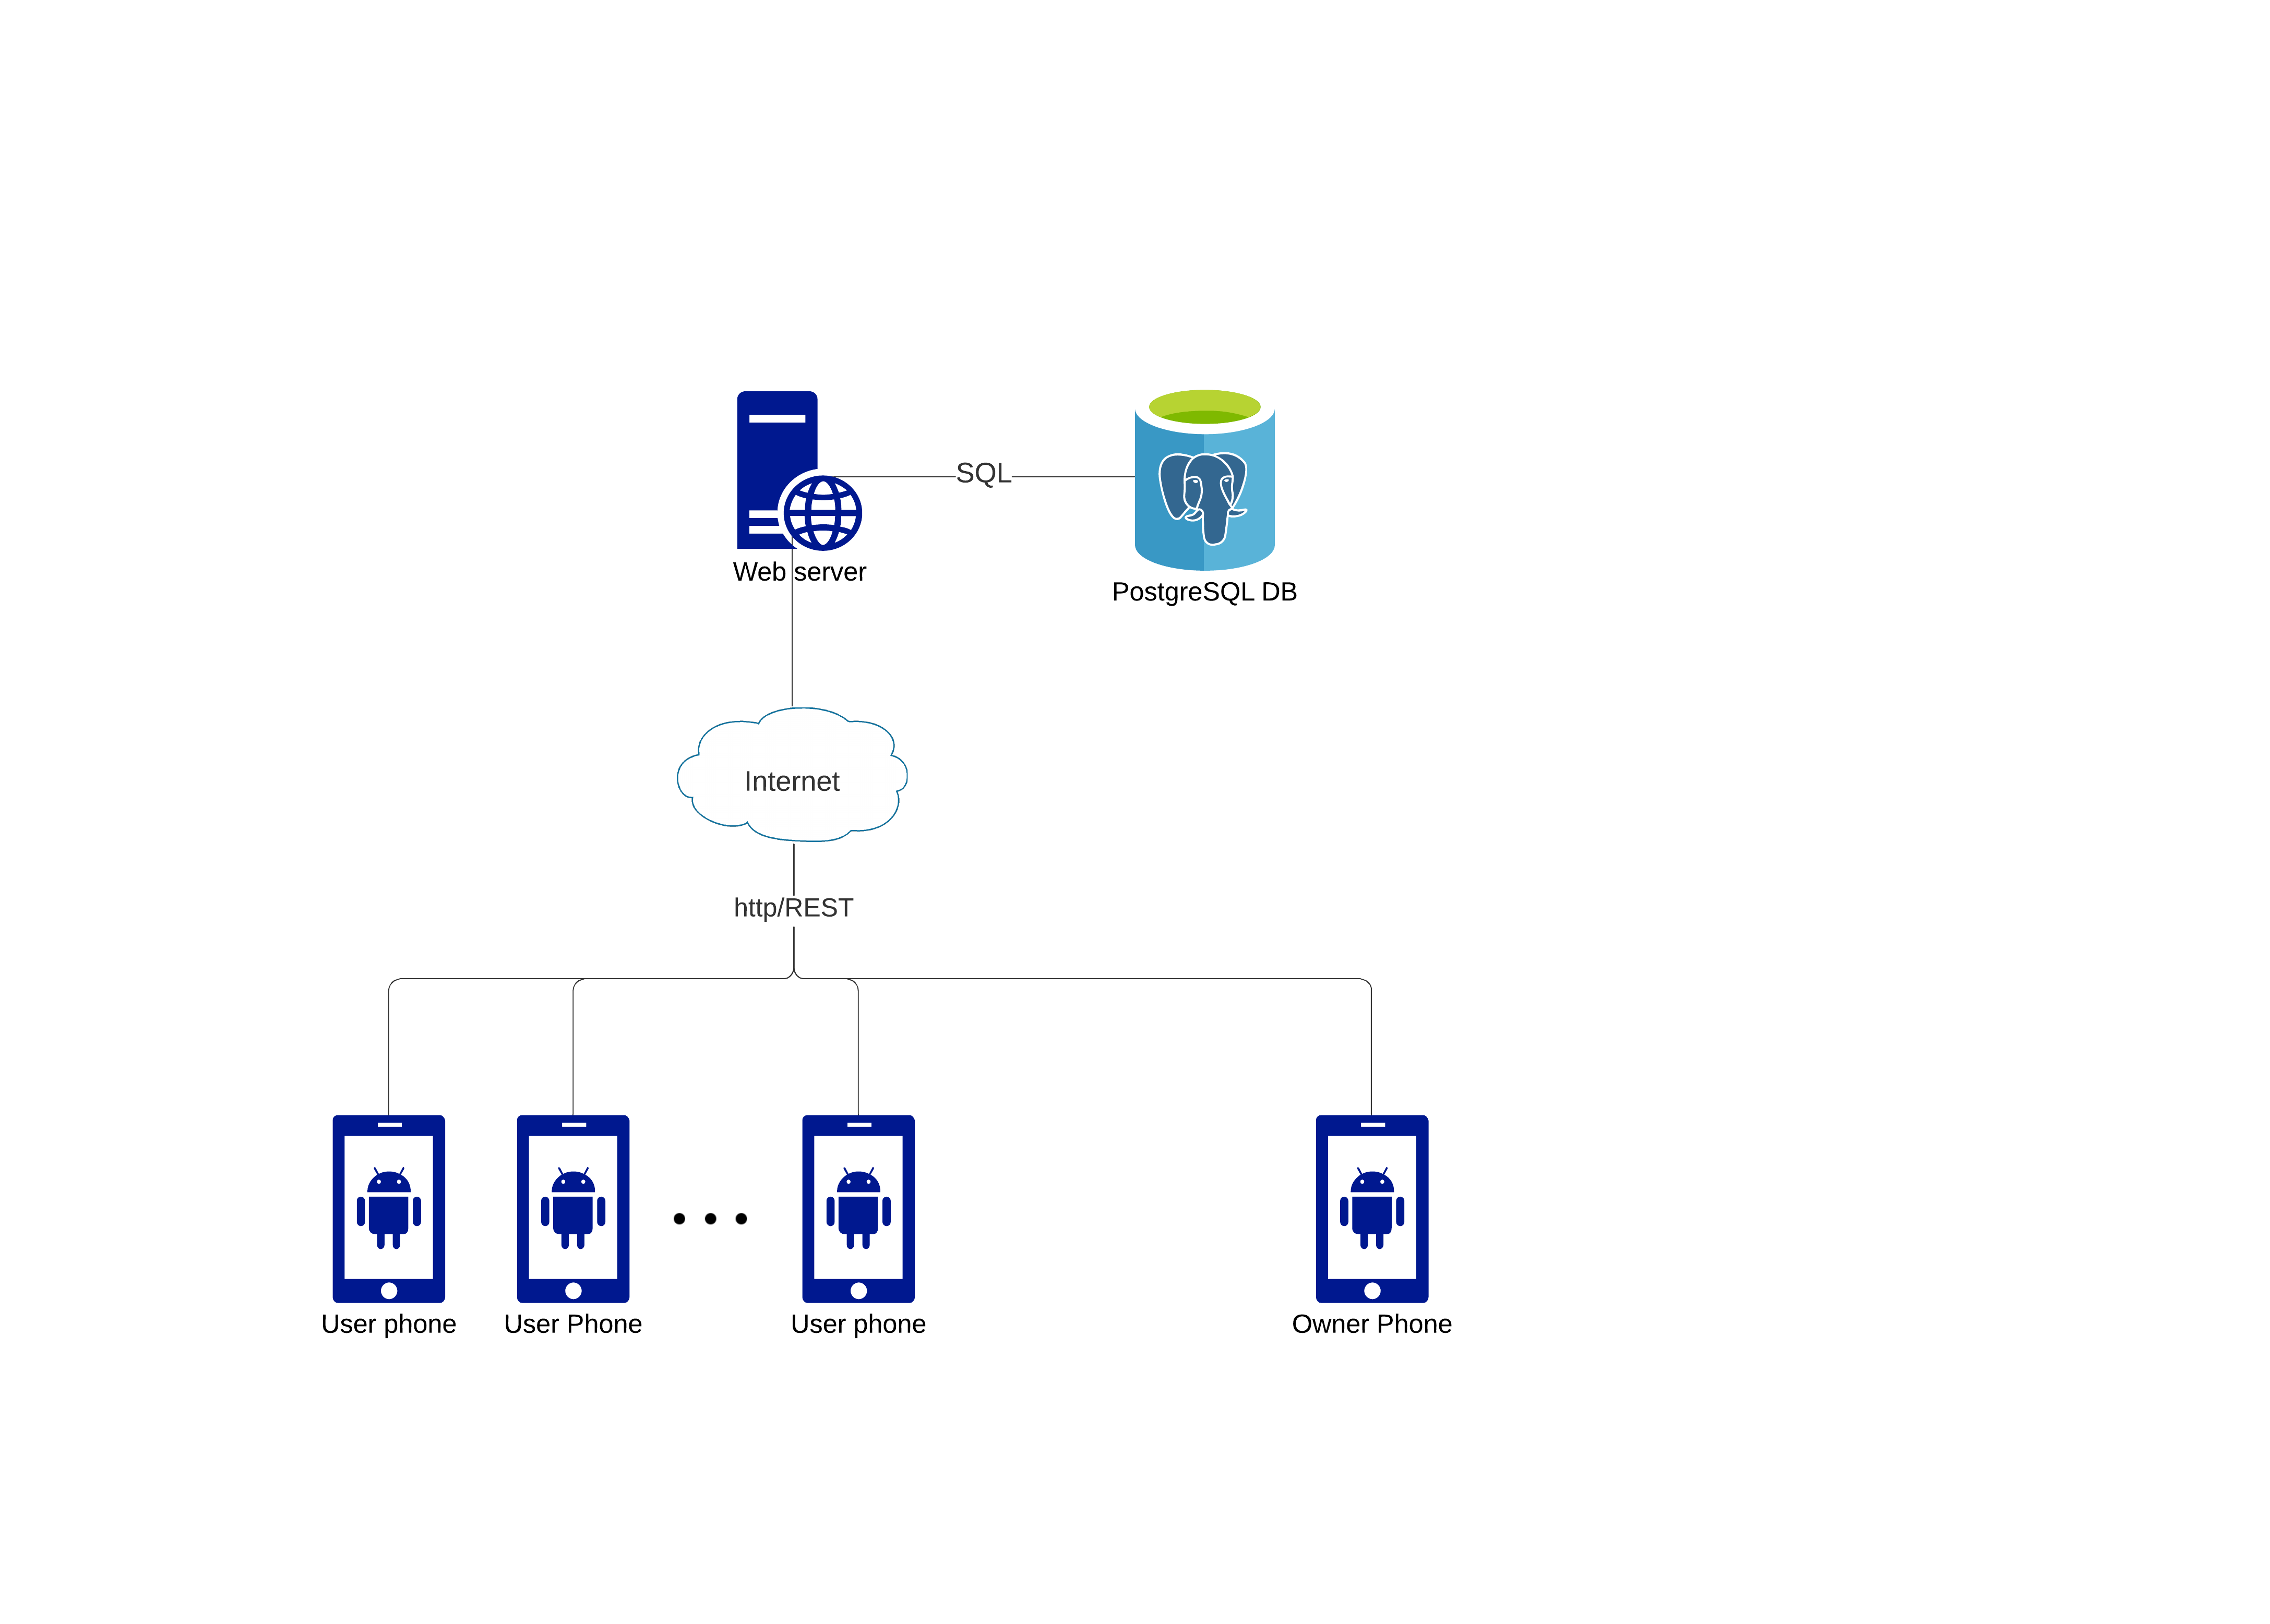
\includegraphics[width=\textwidth]{Topologia_v2.png}
    \caption{Topologia del sistema.}\label{fig:topologia}
\end{figure}